\documentclass{article}
\usepackage[utf8]{inputenc}
\usepackage{amsmath}
\usepackage[english]{babel}
\usepackage{tikz}
\usetikzlibrary{arrows,automata}

\title{CS355 Worksheet 1}
\author{Joshua Williams - 19507359}
\date{February 2023}

\begin{document}

\maketitle

\section{DFA Definition}
\subsection{Two DFAs}
\subsubsection{$M_1$}

\begin{itemize}
  \item What is the start state ?\\ $q_1$.
  
  \item What is the set of accept states?\\ \{\:$q_2$\:\}
  
  \item What sequence of states does the machine go through on input aabb?\\ \{ $q_1 \:\underrightarrow{a} \:q_2 \:\underrightarrow{a} \:q_3 \:\underrightarrow{b} \:q_1 
  \:\underrightarrow{b} \:\underline{q_1}$\:\}
  
  \item Does the machine accept the string aabb ?\\ No.
  \item Does the machine accept the string $\epsilon$ \:?\\ No.
  
\end{itemize}

\subsubsection{$M_2$}
\begin{itemize}
  \item What is the start state ?\\ {$q_1$}.
  
  \item What is the set of accept states?\\ \{\:{$q_1$}, \:{$q_4$}\:\}
  
  \item What sequence of states does the machine go through on input aabb?\\ \{ {$q_1$ \:\underrightarrow{a} \:$q_1$ \:\underrightarrow{a} \:$q_1$ \:\underrightarrow{b} \:$q_2$ 
  \:\underrightarrow{b} \:\underline{$q_4$}} \: \}
  
  \item Does the machine accept the string aabb ?\\ Yes.
  
  \item Does the machine accept the string $\epsilon$ \:?\\ Yes.
\end{itemize}

\subsection{Formal Descriptions}
\subsubsection{$M_1$}

\begin{itemize}
  \item Q = \{ $q_1$, $q_2$, $q_3$ \}
  \item $\Sigma$ = \{ a,b \}
  \item $\delta$ = 
  \begin{displaymath}
  \begin{array}{c|c c}
       & a & b \\
       \hline
      q_1 & q_2 & q_1\\
      q_2 & q_3 & q_3\\
      q_3 & q_2 & q_1
  \end{array}
  \end{displaymath}
  \item $q_0$ = $q_1$
  \item F = \{ $q_2$ \}
\end{itemize}

\subsubsection{$M_2$}

\begin{itemize}
  \item Q = \{ $q_1$, $q_2$, $q_3$, $q_4$ \}
  \item $\Sigma$ = \{ a,b \}
  \item $\delta$ = 
  \begin{displaymath}
  \begin{array}{c|c c}
       & a & b \\
       \hline
      q_1 & q_1 & q_2\\
      q_2 & q_3 & q_4\\
      q_3 & q_2 & q_1\\
      q_4 & q_3 & q_4
  \end{array}
  \end{displaymath}
  \item $q_0$ = $q_1$
  \item F = \{ $q_1$, $q_4$ \}
\end{itemize}

\subsection{DFA Construct}

\begin{tikzpicture}[->,>=stealth',shorten >=1pt,auto,node distance=4cm,
  scale = 1,transform shape]

\node[state] (q_1) [above left of=q_2] {$q_1$};
\node[state] (q_2) [above of=q_3] {$q_2$};
\node[state,accepting,initial] (q_3) {$q_3$};
\node[state] (q_4) [right of=q_3] {$q_4$};
\node[state] (q_5) [above of=q_4] {$q_5$};

\path [-stealth, thick]
  (q_1) edge [loop above] node  {$u$} (q_1)
  (q_1) edge [bend left=1cm] node {$d$} (q_2)
  (q_2) edge [bend left=0.2cm] node {$u$} (q_1)
  (q_2) edge [bend left=0.8cm] node {$d$} (q_3)
  (q_3) edge [bend left=0.4cm] node {$u$} (q_2)
  (q_3) edge [bend left] node {$d$} (q_4)
  (q_4) edge [bend left] node {$u$} (q_3)
  (q_4) edge [bend left] node {$d$} (q_5)
  (q_5) edge [bend left] node {$u$} (q_4)
  (q_5) edge [loop above] node {$d$} (q_5);

\end{tikzpicture}

\section{DFA Exercise}

\subsection{}
  \begin{displaymath}
    \begin{array}{c|c c c}
        & 1 & 2 & 3 \\
         \hline
        f_1 & x & x & x\\
        f_2 & x & x & y\\
        f_3 & x & y & x\\
        f_4 & y & x & x\\
        f_5 & x & y & y\\
        f_6 & y & y & x\\
        f_7 & y & x & y\\
        f_8 & x & y & x\\
        f_9 & y & y & y
    \end{array}
    \end{displaymath}
\subsection{}
Num of states = s = 4 \\
Size of alphabet = a = 3 \\
$s*s^{as}*2^s = ans$ \\
$4*4^{3*4}*2^4 = 1073741824$
\subsection{}
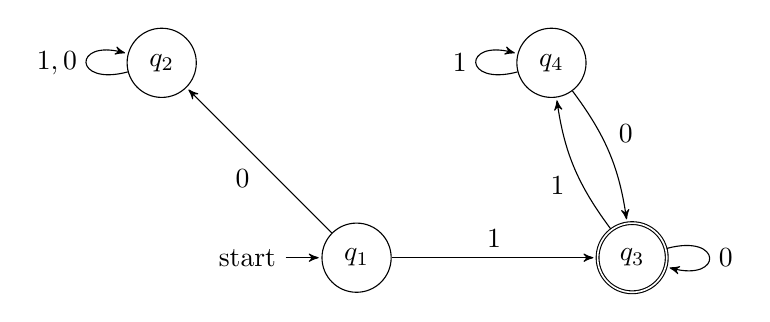
\begin{tikzpicture}[->,>=stealth',shorten >=1pt,auto,node distance=3.5cm,
    scale = 1,transform shape]

  \node[state,initial] (q_1) {$q_1$};
  \node[state] (q_2) [above left of=q_1] {$q_2$};
  \node[state,accepting] (q_3) [right of=q_1] {$q_3$};
  \node[state] (q_4) [above right of=q_1] {$q_4$};

  \path (q_1) edge node {$0$} (q_2)
      (q_2) edge [loop left] node {$1, 0$} (q_2)
      (q_1) edge              node {$1$} (q_3)
      (q_3) edge [bend left=0.5cm] node {$1$} (q_4)
      (q_3) edge [loop right] node {$0$} (q_3)
      (q_4) edge [bend left=0.5cm] node {$0$} (q_3)
      (q_4) edge [loop left] node {$1$} (q_4);

  \end{tikzpicture}
\subsection{}
\begin{tikzpicture}[->,>=stealth',shorten >=1pt,auto,node distance=3.5cm,
  scale = 1,transform shape]

\node[state,initial] (q_1) [n/a of=] {$q_1$};
\node[state] (q_2) [right of=q_1] {$q_2$};
\node[state] (q_3) [right of=q_2] {$q_3$};
\node[state,accepting] (q_4) [below right of=q_2] {$q_4$};

\path (q_1) edge [loop above] node {$0$} (q_1)
  (q_1) edge              node {$1$} (q_2)
  (q_2) edge [loop above] node {$0$} (q_2)
  (q_2) edge              node {$1$} (q_3)
  (q_3) edge [loop above] node {$0$} (q_3)
  (q_3) edge              node {$1$} (q_4)
  (q_4) edge [loop left] node {$0, 1$} (q_4);

\end{tikzpicture}
\subsection{}
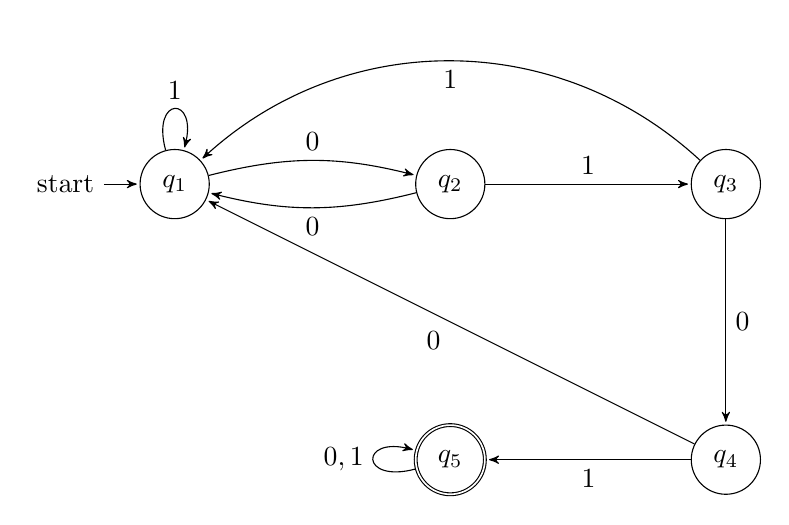
\begin{tikzpicture}[->,>=stealth',shorten >=1pt,auto,node distance=3.5cm,
  scale = 1,transform shape]

\node[state,initial] (q_1) {$q_1$};
\node[state] (q_2) [right of=q_1] {$q_2$};
\node[state] (q_3) [right of=q_2] {$q_3$};
\node[state] (q_4) [below of=q_3] {$q_4$};
\node[state,accepting] (q_5) [left of=q_4] {$q_5$};

\path (q_1) edge [loop above] node {$1$} (q_1)
  (q_1) edge [bend left=0.5cm] node {$0$} (q_2)
  (q_2) edge [bend left=0.5cm] node {$0$} (q_1)
  (q_2) edge              node {$1$} (q_3)
  (q_3) edge [bend right=1.5cm] node {$1$} (q_1)
  (q_3) edge              node {$0$} (q_4)
  (q_4) edge              node {$0$} (q_1)
  (q_4) edge              node {$1$} (q_5)
  (q_5) edge [loop left] node {$0, 1$} (q_5);

\end{tikzpicture}
\subsection{}
\begin{tikzpicture}[->,>=stealth',shorten >=1pt,auto,node distance=3.5cm,
  scale = 1,transform shape]

\node[state,initial] (q_1) {$q_1$};
\node[state] (q_2) [right of=q_1] {$q_2$};
\node[state] (q_3) [right of=q_2] {$q_3$};
\node[state,accepting] (q_4) [below of=q_3] {$q_4$};
\node[state] (q_5) [above of=q_3] {$q_5$};

\path (q_1) edge              node {$0, 1$} (q_2)
  (q_2) edge              node {$0, 1$} (q_3)
  (q_3) edge              node {$0$} (q_4)
  (q_4) edge [loop left] node {$0, 1$} (q_4)
  (q_3) edge              node {$1$} (q_5)
  (q_5) edge [loop left] node {$0, 1$} (q_5);

\end{tikzpicture}
\subsection{}
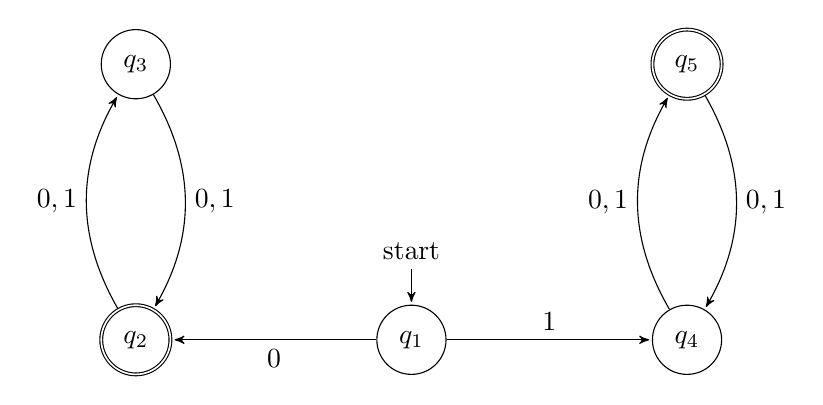
\begin{tikzpicture}[->,>=stealth',shorten >=1pt,auto,node distance=3.5cm,
  scale = 1,transform shape]

\node[state,initial above] (q_1) {$q_1$};
\node[state,accepting] (q_2) [left of=q_1] {$q_2$};
\node[state] (q_3) [above of=q_2] {$q_3$};
\node[state] (q_4) [right of=q_1] {$q_4$};
\node[state,accepting] (q_5) [above of=q_4] {$q_5$};

\path (q_1) edge              node {$0$} (q_2)
  (q_1) edge              node {$1$} (q_4)
  (q_2) edge [bend left] node {$0, 1$} (q_3)
  (q_3) edge [bend left]  node {$0, 1$} (q_2)
  (q_4) edge [bend left]  node {$0, 1$} (q_5)
  (q_5) edge [bend left]  node {$0, 1$} (q_4);

\end{tikzpicture}
\subsection{}
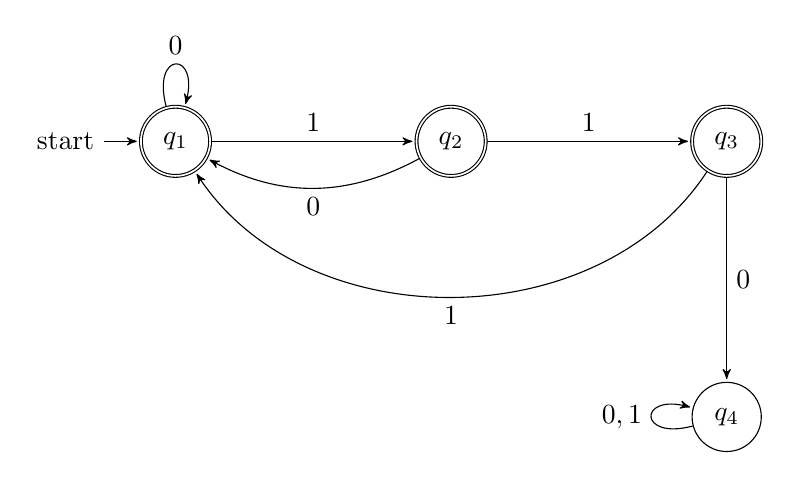
\begin{tikzpicture}[->,>=stealth',shorten >=1pt,auto,node distance=3.5cm,
  scale = 1,transform shape]

\node[state,accepting,initial] (q_1) {$q_1$};
\node[state,accepting] (q_2) [right of=q_1] {$q_2$};
\node[state,accepting] (q_3) [right of=q_2] {$q_3$};
\node[state] (q_4) [below of=q_3] {$q_4$};

\path (q_1) edge [loop above] node {$0$} (q_1)
  (q_1) edge              node {$1$} (q_2)
  (q_2) edge [bend left=1cm] node {$0$} (q_1)
  (q_2) edge              node {$1$} (q_3)
  (q_3) edge [bend left=2cm] node {$1$} (q_1)
  (q_3) edge              node {$0$} (q_4)
  (q_4) edge [loop left] node {$0, 1$} (q_4);

\end{tikzpicture}

\subsection{}
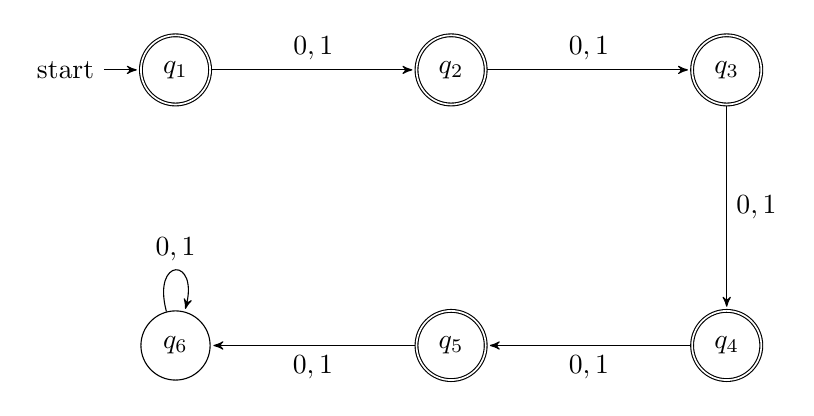
\begin{tikzpicture}[->,>=stealth',shorten >=1pt,auto,node distance=3.5cm,
  scale = 1,transform shape]

\node[state,accepting,initial] (q_1) {$q_1$};
\node[state,accepting] (q_2) [right of=q_1] {$q_2$};
\node[state,accepting] (q_3) [right of=q_2] {$q_3$};
\node[state,accepting] (q_4) [below of=q_3] {$q_4$};
\node[state,accepting] (q_5) [left of=q_4] {$q_5$};
\node[state] (q_6) [left of=q_5] {$q_6$};

\path (q_1) edge              node {$0, 1$} (q_2)
  (q_2) edge              node {$0, 1$} (q_3)
  (q_3) edge              node {$0, 1$} (q_4)
  (q_4) edge              node {$0, 1$} (q_5)
  (q_5) edge              node {$0, 1$} (q_6)
  (q_6) edge [loop above] node {$0, 1$} (q_6);

\end{tikzpicture}

\subsection{}
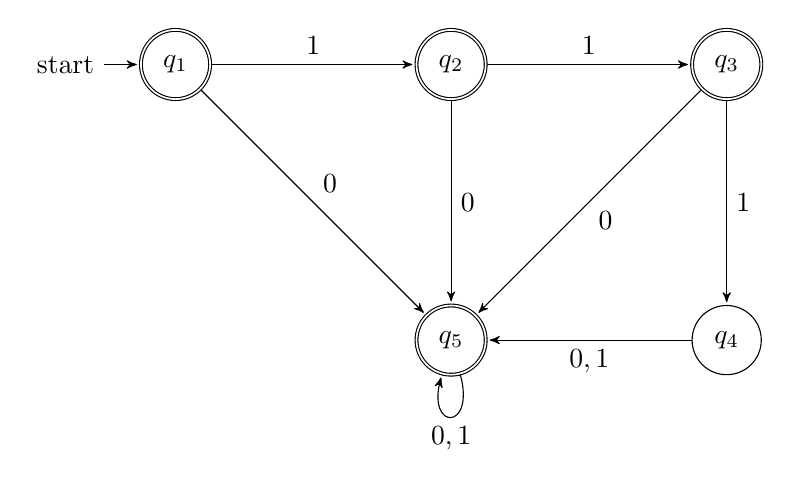
\begin{tikzpicture}[->,>=stealth',shorten >=1pt,auto,node distance=3.5cm,
  scale = 1,transform shape]

\node[state,accepting,initial] (q_1) {$q_1$};
\node[state,accepting] (q_2) [right of=q_1] {$q_2$};
\node[state,accepting] (q_3) [right of=q_2] {$q_3$};
\node[state] (q_4) [below of=q_3] {$q_4$};
\node[state,accepting] (q_5) [below of=q_2] {$q_5$};

\path (q_1) edge              node {$1$} (q_2)
  (q_2) edge              node {$1$} (q_3)
  (q_3) edge              node {$1$} (q_4)
  (q_4) edge              node {$0, 1$} (q_5)
  (q_5) edge [loop below] node {$0, 1$} (q_5)
  (q_1) edge              node {$0$} (q_5)
  (q_2) edge              node {$0$} (q_5)
  (q_3) edge              node {$0$} (q_5);

\end{tikzpicture}

\end{document}
